\chapter{Appendix}

\begin{figure}[htbp]
  % \begin{subfigure}{0.95\textwidth}
  %   \centering
  %   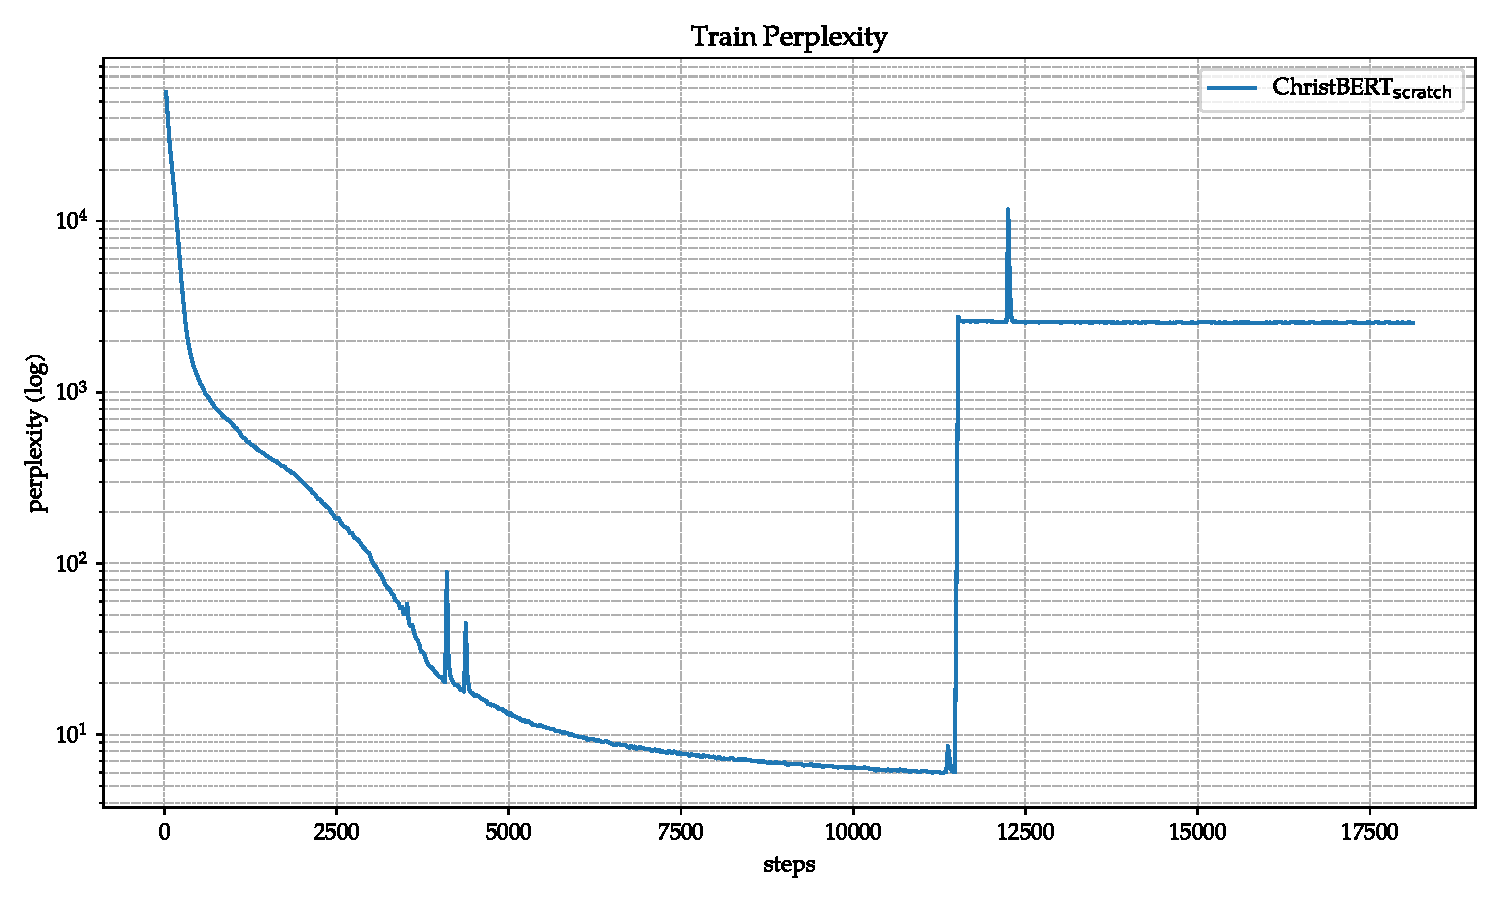
\includegraphics[width=\textwidth]{div_ppl_train}
  %   \caption{Perplexity on training set}
  % \end{subfigure}
  % \begin{subfigure}{0.95\textwidth}
  %   \centering
  %   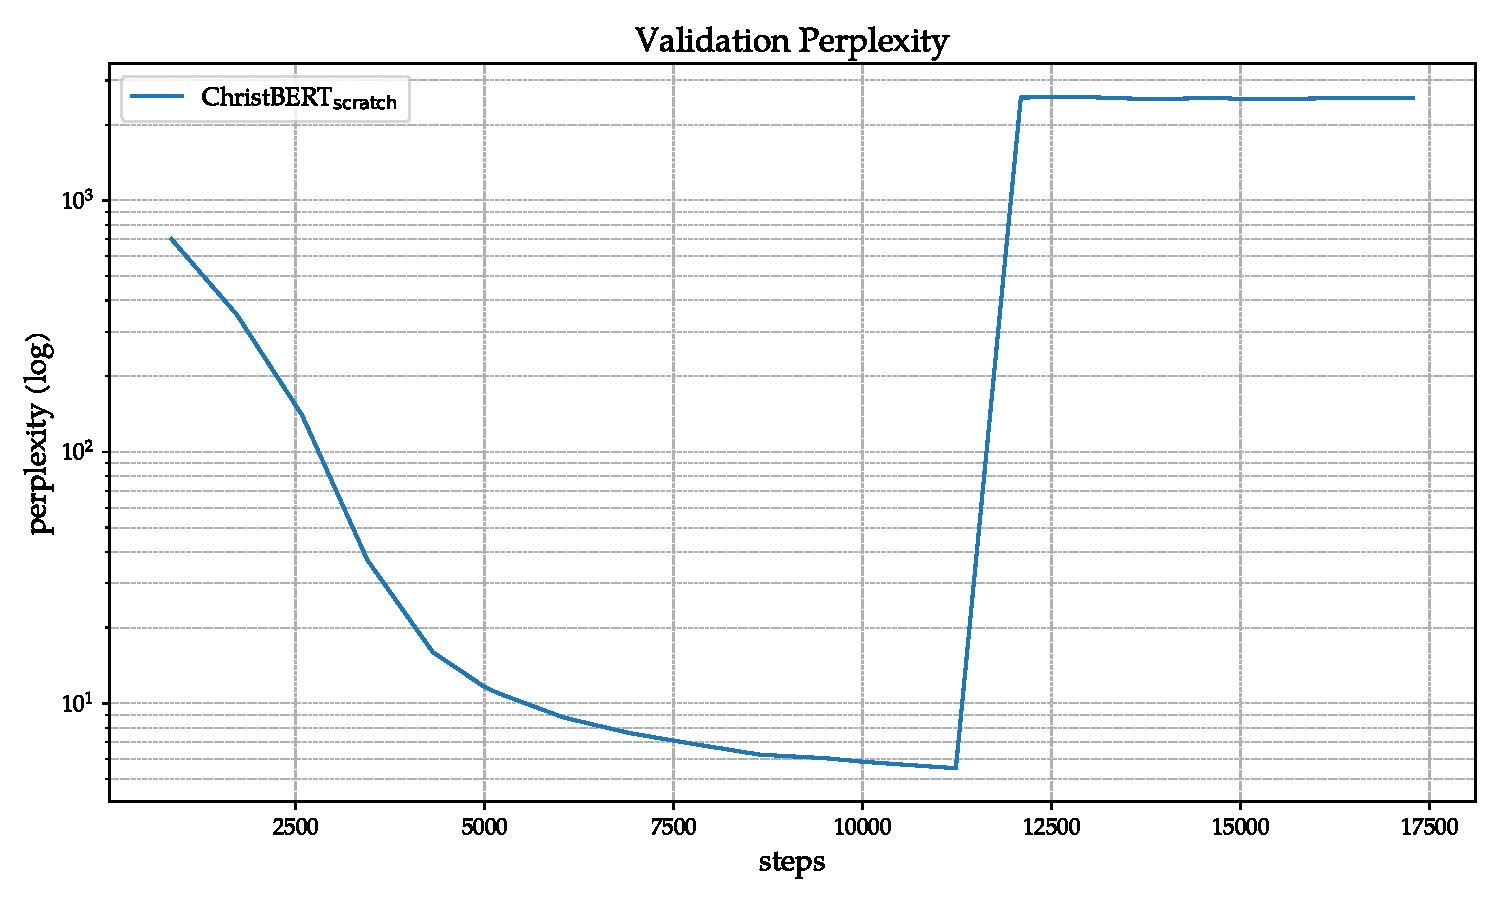
\includegraphics[width=\textwidth]{div_ppl_val}
  %   \caption{Perplexity on validation set}
  % \end{subfigure}
  \centering
  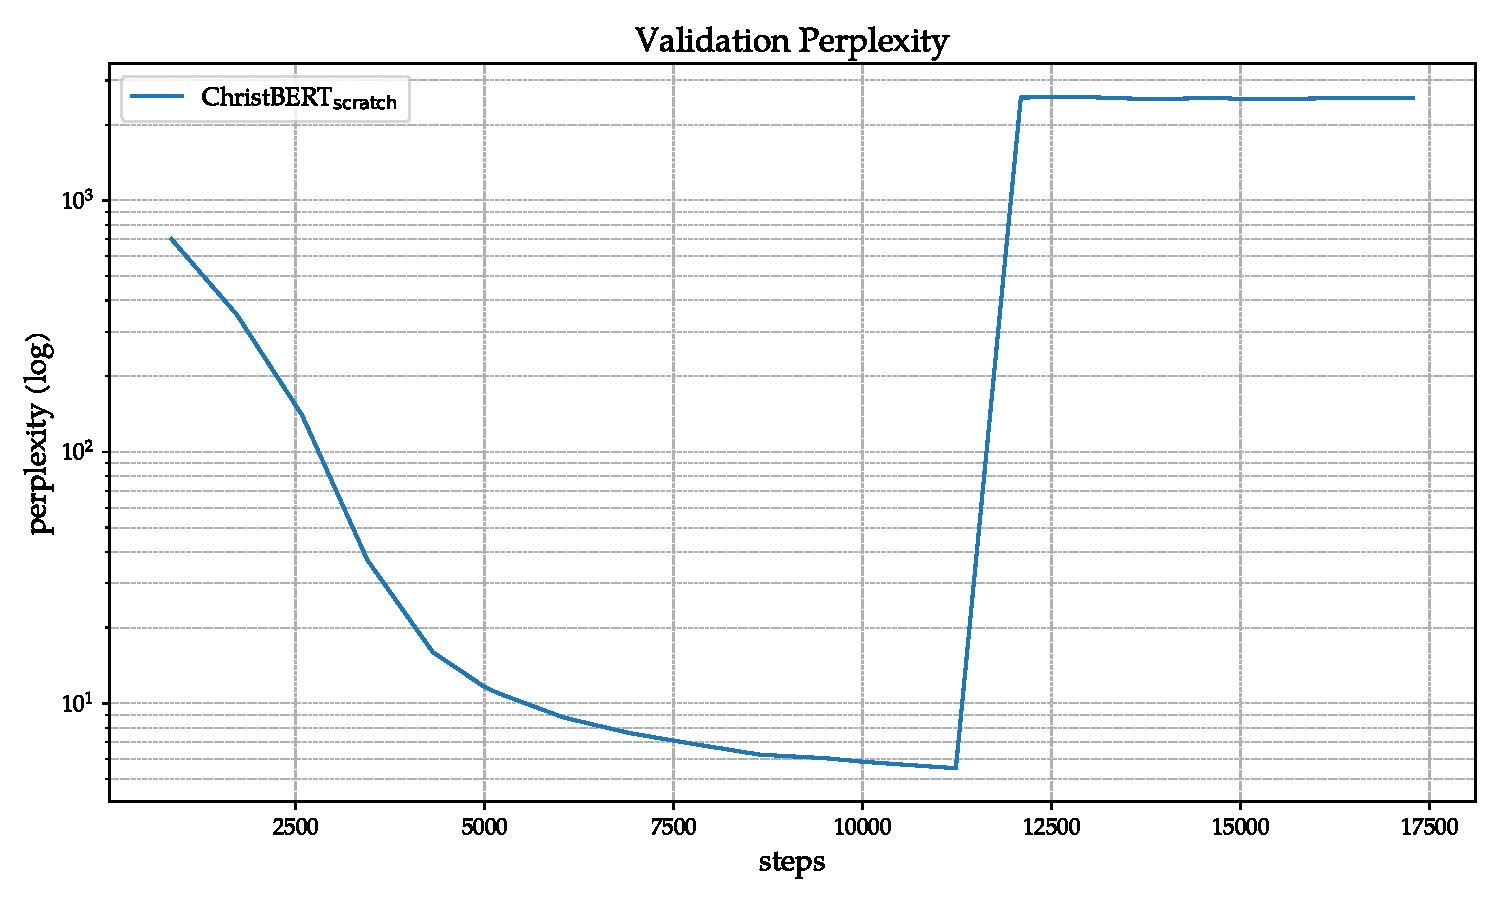
\includegraphics[width=0.95\textwidth]{div_ppl_val}
  \caption[Perplexity during diverged pre-training of
  \ChristBERT\textsubscript{scratch}]{Perplexity during diverged pre-training of
  \ChristBERT\textsubscript{scratch}. Perplexity is shown in log scale for every
  optimization step and evaluated on the validation split of the pre-training
  corpus. The plot illustrates a sharp increase in perplexity around the
  12,500th step, indicating model instability and failure to converge.}
  \label{fig:div_ppl}
\end{figure}

\begin{table}[htb] 
  \centering 
  \begin{tabular}{l cc}
    \toprule
    \bfseries Model & \bfseries Vocab Size & \bfseries \# Parameters \\ 
    \midrule
    \ChristBERT & 52,009 & 125,985,024 \\
    \ChristBERT\textsubscript{scratch} & 52,009 & 125,985,024 \\
    \ChristBERT\textsubscript{BPE} & 52,009 & 125,985,024 \\
    medBERT.de & 30,000 & 109,081,344 \\
    BioGottBERT & 52,009 & 125,985,024 \\
    GeistBERT & 52,009 & 125,985,024 \\
    GeBERTa & 50,266 & 138,620,928 \\
    \bottomrule
\end{tabular}

  \caption[Vocabulary size and parameter size of evaluated models]{The
  vocabulary size and parameter size are shown for the evaluated models. This
  table does not show other design differences of the models. Values extracted
  using \textsc{Huggingface Transformers} library~\cite{wolf2020transformers}.}
  \label{tab:model_props}
\end{table}

\begin{table}[htb]
    \centering
    \begin{tabular}{lclcc}
    \toprule
    \multirow{2}{*}{\bfseries Model} &
    \bfseries Computation Time &
    \multicolumn{2}{c}{\multirow{2}{*}{\bfseries GPUs}} &
    \multirow{2}{*}{\bfseries VRAM} \\
    & (DD:HH:MM) & & & \\
    \midrule
    \ChristBERT{} & 6:20:09 & 4 $\times$ A100 SXM && 80 GB \\
    \ChristBERT\textsubscript{scratch} & 6:19:13 & 4 $\times$ A100 SXM && 80 GB \\
    \ChristBERT\textsubscript{BPE} & 7:09:12 & 2 $\times$ H100 && 93 GB \\
    \bottomrule
\end{tabular}

    \caption[Computation time of pre-training]{Pre-training computation time in
    days, hours and minutes summing up to 521 hours and 54 minutes, which are
    approximately 21.74 days.}
    \label{tab:train_gpu_time}
\end{table}

\begin{table}[htbp]
    \centering
    % Prompt: Fill in the values in the tex table. The column for the values in the csv are train_runtime for FT and total_runtime for PT . Format FT as hh:mm:ss (round up seconds). The values belong in the tex table with row model_name and column data_name.

\begin{tabular}{l ccccc}
    \toprule
    \bfseries Model & \bfseries BRONCO150 & \bfseries CARDIO:DE & 
    \bfseries GGPONC & \bfseries CLEF & \bfseries JSynCC \\
    \midrule
    \ChristBERT & 1:20:26 & 4:40:01 & 11:26:14 & 11:24:22 & 2:10:02 \\
    \ChristBERT\textsubscript{scratch} & 1:28:28 & 5:14:12 & 10:47:27 & 12:16:22 & 2:30:59 \\
    \ChristBERT\textsubscript{BPE} & 1:12:09 & 4:55:18 & 10:51:00 & 11:45:43 & 2:25:13 \\
    medBERT.de & 1:57:32 & 4:31:53 & 11:25:21 & 12:53:27 & 2:13:56 \\
    BioGottBERT & 1:18:15 & 6:01:10 & 10:55:55 & 12:50:17 & 2:03:28 \\
    GeistBERT & 1:27:57 & 4:40:46 & 11:25:43 & 12:51:41 & 2:15:12 \\
    GeBERTa & 1:57:32 & 7:39:51 & 19:22:22 & 29:15:23 & 3:09:10 \\
    \bottomrule
\end{tabular}

    \caption[Computation time of hyperparameter grid search]{Computation time in
    hours, minutes and seconds spent on the hyperparameter grid search for
    finding the best models for each task. The grid search was performed on a
    single NVIDIA RTX 3090 GPU with 24 GB VRAM. The total computation time for
    hyperparameter optimization sums up to 161 hours and 46 minutes, which are
    approximately 6.74 days.}
    \label{tab:eval_total_time}
\end{table}

\begin{table}[htbp]
    \centerline{ 
    % Prompt: Fill in the values in the tex table. The column for the subcolumn values in the csv are train_runtime for FT and predict_runtime for PT . Format FT as mm:ss (round up seconds) and PT as ss.ss. The values belong in the tex table with row model_name and column data_name.

\begin{tabular}{l cc cc cc cc cc}
    \toprule
    \multirow{2}{*}[-0.5\dimexpr \aboverulesep + \belowrulesep + \cmidrulewidth]{\bfseries Model} &
    \multicolumn{2}{c}{\bfseries BRONCO150} &
    \multicolumn{2}{c}{\bfseries CARDIO:DE} &
    \multicolumn{2}{c}{\bfseries GGPONC} &
    \multicolumn{2}{c}{\bfseries CLEF} &
    \multicolumn{2}{c}{\bfseries JSynCC} \\
    \cmidrule(lr){2-3} \cmidrule(lr){4-5} \cmidrule(lr){6-7} \cmidrule(lr){8-9} \cmidrule(lr){10-11}
    & FT & PT & FT & PT & FT & PT & FT & PT & FT & PT \\
    \midrule
    \ChristBERT & 03:51 & 0.13 & 18:27 & 1.30 & 30:06 & 5.08 & 26:33 & 0.91 & 03:05 & 0.18 \\
    \ChristBERT\textsubscript{scratch} & 02:40 & 0.11 & 15:16 & 0.87 & 30:03 & 5.14 & 29:51 & 0.94 & 06:19 & 0.18 \\
    \ChristBERT\textsubscript{BPE} & 02:03 & 0.13 & 11:09 & 1.01 & 24:53 & 5.45 & 26:32 & 1.08 & 07:16 & 0.39 \\
    medBERT.de & 04:17 & 0.13 & 08:07 & 0.95 & 25:32 & 5.81 & 27:30 & 1.06 & 04:56 & 0.21 \\
    BioGottBERT & 05:46 & 0.11 & 16:48 & 0.92 & 32:47 & 5.14 & 29:13 & 1.05 & 05:28 & 0.19 \\
    GeistBERT & 04:05 & 0.19 & 15:14 & 0.88 & 29:57 & 4.83 & 29:45 & 0.96 & 04:09 & 0.19 \\
    GeBERTa & 04:17 & 0.13 & 28:47 & 1.36 & 49:41 & 7.23 & 56:48 & 2.05 & 06:11 & 0.41 \\
    \bottomrule
\end{tabular}
} 
    \caption[Computation time of fine-tuning and inference]{Fine-tuning (FT)
    runtime in minutes and seconds, and prediction runtime (PT) in seconds of
    the best downstream task models for each task. Both were performed on one
    NVIDIA RTX 3090 GPU with 24 GB VRAM.}
    \label{tab:eval_gpu_time}
\end{table}

\begin{table}[htbp]
    \centerline{
    % Prompt: Fill in the values in the tex table. The column for the subcolumn values in the csv are batch_size for BS and learning_rate for LR. Enclose LR in \num{} i.e \num{7e-5}.  The values belong in the tex table with row model_name and column data_name.

\begin{tabular}{l cc cc cc cc cc}
    \toprule
    \multirow{2}{*}[-0.5\dimexpr \aboverulesep + \belowrulesep + \cmidrulewidth]{\bfseries Model} & 
    \multicolumn{2}{c}{\bfseries BRONCO150} &
    \multicolumn{2}{c}{\bfseries CARDIO:DE} &
    \multicolumn{2}{c}{\bfseries GGPONC} &
    \multicolumn{2}{c}{\bfseries CLEF} &
    \multicolumn{2}{c}{\bfseries JSynCC} \\
    \cmidrule(lr){2-3} \cmidrule(lr){4-5} \cmidrule(lr){6-7} \cmidrule(lr){8-9} \cmidrule(lr){10-11}
    & BS & LR & BS & LR & BS & LR & BS & LR & BS & LR \\
    \midrule
    \ChristBERT & 48 & \num{7e-5} & 48 & \num{7e-5} & 16 & \num{7e-5} & 16 & \num{5e-5} & 48 & \num{5e-5} \\
    \ChristBERT\textsubscript{scratch} & 32 & \num{5e-5} & 16 & \num{5e-5} & 16 & \num{7e-5} & 16 & \num{2e-5} & 64 & \num{5e-5} \\
    \ChristBERT\textsubscript{BPE} & 32 & \num{7e-5} & 32 & \num{5e-5} & 32 & \num{7e-5} & 16 & \num{7e-5} & 16 & \num{5e-6} \\
    medBERT.de & 16 & \num{5e-5} & 48 & \num{7e-5} & 32 & \num{5e-5} & 32 & \num{7e-5} & 64 & \num{2e-5} \\
    BioGottBERT & 16 & \num{7e-5} & 16 & \num{5e-5} & 16 & \num{7e-5} & 16 & \num{7e-5} & 16 & \num{7e-5} \\
    GeistBERT & 16 & \num{2e-5} & 16 & \num{5e-5} & 16 & \num{5e-5} & 16 & \num{2e-5} & 16 & \num{7e-5} \\
    GeBERTa & 16 & \num{5e-5} & 16 & \num{7e-5} & 16 & \num{5e-5} & 48 & \num{7e-5} & 32 & \num{5e-5} \\
    \bottomrule
\end{tabular}
}
    \caption[Best hyperparameters found in the grid search for the downstream
    tasks]{Hyperparameters of the best downstream task models for each task and
    pre-trained model. BS and LR denote batch size and learning rate,
    respectively.}
    \label{tab:best_hyperparams}
\end{table}

\begin{table}[htbp]
  \centering
  % Prompt: Fill in the values in the tex table. The column for the column values in the csv is predict_[entity]_(prediction, recall, \ff). Format the values in percent without the symbols i.e. xx.xx. The values belong in the tex table with row model_name.

\begin{tabular}{l ccc ccc ccc}
    \toprule
    \multirow{2}{*}[-0.5\dimexpr \aboverulesep + \belowrulesep + \cmidrulewidth]{\bfseries Model} &
    \multicolumn{3}{c}{\bfseries Diagnosis} &
    \multicolumn{3}{c}{\bfseries Medication} &
    \multicolumn{3}{c}{\bfseries Treatment} \\
    \cmidrule(lr){2-4} \cmidrule(lr){5-7} \cmidrule(lr){8-10}
    & Prec. & Rec. & \ff & 
    Prec. & Rec. & \ff & 
    Prec. & Rec. & \ff \\
    \midrule
    \ChristBERT & \underline{79.78} & \textbf{81.56} & \underline{80.66} & 85.71 & 81.36 & 83.48 & 81.89 & 83.87 & 82.87 \\
    \ChristBERT\textsubscript{scratch} & 78.89 & 79.33 & 79.11 & \underline{87.50} & 83.05 & \underline{85.22} & \underline{83.59} & \underline{86.29} & \underline{84.92} \\
    \ChristBERT\textsubscript{BPE} & \textbf{82.63} & \underline{80.00} & \textbf{81.29} & \textbf{88.41} & 84.72 & \textbf{86.52} & \textbf{88.82} & \textbf{88.82} & \textbf{88.82} \\
    medBERT.de & 75.35 & 75.35 & 75.35 & 85.71 & 83.33 & 84.51 & 80.13 & 84.03 & 82.03 \\
    BioGottBERT & 72.07 & 72.07 & 72.07 & 83.33 & \underline{84.75} & 84.03 & 80.77 & 84.68 & 82.68 \\
    GeistBERT & 74.05 & 76.54 & 75.27 & 81.25 & \textbf{88.14} & 84.55 & 75.19 & 80.65 & 77.82 \\
    GeBERTa & 75.35 & 75.35 & 75.35 & 85.71 & 83.33 & 84.51 & 80.13 & 84.03 & 82.03 \\
    \bottomrule
\end{tabular}
  
  \caption[Overview of per entity precision, recall and \ff{} scores achieved on
  the BRONCO150 dataset]{Overview of per entity precision (Prec.), recall (Rec.)
  and \ff{} scores achieved on the BRONCO150 dataset All results are shown in
  percent and assess each model's best fine-tuned performance on the test set.
  The best model was selected out of 28 runs based on its validation set
  performance. Best score in bold and second best underlined.}
  \label{tab:bronco}
\end{table}

\begin{table}[htbp]
  \centering
  % Prompt: Fill in the values in the tex table. The column for the column values in the csv is predict_[entity]_(prediction, recall, \ff). Format the values in percent without the symbols i.e. xx.xx. The values belong in the tex table with row model_name.

\begin{tabular}{l ccc ccc ccc}
    \toprule
    \multirow{2}{*}[-0.5\dimexpr \aboverulesep + \belowrulesep + \cmidrulewidth]{\bfseries Model} &
    \multicolumn{3}{c}{\bfseries ActiveIng} &
    \multicolumn{3}{c}{\bfseries Drug} &
    \multicolumn{3}{c}{\bfseries Duration} \\
    \cmidrule(lr){2-4} \cmidrule(lr){5-7} \cmidrule(lr){8-10}
    & Prec. & Rec. & \ff &
    Prec. & Rec. & \ff &
    Prec. & Rec. & \ff \\
    \midrule
    \ChristBERT & 85.71 & \textbf{92.96} & \underline{89.19} & 84.85 & 86.15 & 85.50 & 50.00 & \underline{60.00} & 54.55 \\
    \ChristBERT\textsubscript{scratch} & 85.62 & 90.14 & 87.82 & 84.38 & 83.08 & 83.72 & \textbf{59.26} & 58.18 & \underline{58.72} \\
    \ChristBERT\textsubscript{BPE} & \textbf{88.52} & \underline{92.40} & \textbf{90.41} & \underline{91.14} & \textbf{91.14} & \textbf{91.14} & \underline{58.82} & \textbf{60.61} & \textbf{59.70} \\
    medBERT.de & 85.93 & 90.06 & 87.95 & 88.89 & 88.89 & \underline{88.89} & 46.97 & 49.21 & 48.06 \\
    BioGottBERT & 86.29 & 90.85 & 88.51 & 87.30 & 84.62 & 85.94 & 50.85 & 54.55 & 52.63 \\
    GeistBERT & 84.49 & 90.14 & 87.22 & 79.17 & 87.69 & 83.21 & 45.59 & 56.36 & 50.41 \\
    GeBERTa & \underline{88.24} & 89.55 & 88.89 & \textbf{92.31} & \underline{90.00} & \textbf{91.14} & 55.17 & 50.79 & 52.89 \\
    
    \midrule
    & \multicolumn{3}{c}{\bfseries Form} &
    \multicolumn{3}{c}{\bfseries Frequency} &
    \multicolumn{3}{c}{\bfseries Strength} \\
    \cmidrule(lr){2-4} \cmidrule(lr){5-7} \cmidrule(lr){8-10}
    \ChristBERT & 20.00 & \underline{25.00} & 22.22 & 94.63 & \textbf{96.04} & 95.33 & \underline{97.10} & 95.26 & 96.17 \\
    \ChristBERT\textsubscript{scratch} & \textbf{50.00} & \textbf{50.00} & \textbf{50.00} & 93.10 & 93.56 & 93.33 & \textbf{97.16} & \underline{97.16} & \textbf{97.16} \\
    \ChristBERT\textsubscript{BPE} & 16.67 & \underline{25.00} & 20.00 & 95.06 & 94.29 & 94.67 & 94.94 & 96.06 & 95.50 \\
    medBERT.de & \textbf{50.00} & \textbf{50.00} & \textbf{50.00} & 95.00 & \underline{95.87} & 95.43 & 95.15 & 96.86 & 96.00 \\
    BioGottBERT & \textbf{50.00} & \textbf{50.00} & \textbf{50.00} & \underline{96.04} & \textbf{96.04} & \textbf{96.04} & 95.37 & \textbf{97.63} & \underline{96.49} \\
    GeistBERT & \underline{33.33} & \textbf{50.00} & \underline{40.00} & 93.60 & 94.06 & 93.83 & 96.15 & 94.79 & 95.47 \\
    GeBERTa & \textbf{50.00} & \textbf{50.00} & \textbf{50.00} & \textbf{96.37} & 95.60 & \underline{95.98} & 96.03 & 96.41 & 96.22 \\
    \bottomrule
\end{tabular}
  
  \caption[Overview of per entity precision, recall and \ff{} scores achieved on
  the CARDIO:DE dataset]{Overview of per entity precision (Prec.), recall (Rec.)
  and \ff{} scores achieved on the CARDIO:DE dataset All results are shown in
  percent and assess each model's best fine-tuned performance on the test set.
  The best model was selected out of 28 runs based on its validation set
  performance. Best score in bold and second best underlined.}
  \label{tab:cardiode}
\end{table}

\begin{table}[htbp]
  \centering
  \begin{tabular}{l ccc ccc ccc}
    \toprule
    \multirow{3}{*}[-0.5\dimexpr \aboverulesep + \belowrulesep + \cmidrulewidth]{\bfseries Model} &
    \multicolumn{3}{c}{\multirow{2}{*}{\bfseries Clinical}} &
    \multicolumn{3}{c}{\bfseries Diagnosis /} &
    \multicolumn{3}{c}{\multirow{2}{*}{\bfseries Diagnostic}} \\
    & & & & \multicolumn{3}{c}{\bfseries {Pathology}} & & & \\
    \cmidrule(lr){2-4} \cmidrule(lr){5-7} \cmidrule(lr){8-10}
    & Prec. & Rec. & \ff & Prec. & Rec. & \ff & Prec. & Rec. & \ff \\
    \midrule
    \ChristBERT & 79.12 & \textbf{84.28} & \underline{81.62} & 80.26 & 80.81 & 80.53 & 73.34 & 76.18 & 74.73 \\
    \ChristBERT\textsubscript{scratch} & \underline{79.87} & \underline{83.60} & \textbf{81.69} & 80.35 & \textbf{81.67} & \textbf{81.01} & \textbf{73.78} & 76.82 & \underline{75.27} \\
    \ChristBERT\textsubscript{BPE} & \textbf{80.14} & 82.86 & 81.48 & \textbf{80.66} & \underline{81.31} & \underline{80.98} & \underline{73.62} & \textbf{77.54} & \textbf{75.53} \\
    medBERT.de & 76.29 & 81.02 & 78.58 & 78.46 & 78.88 & 78.67 & 72.09 & 74.19 & 73.13 \\
    BioGottBERT & 79.14 & 80.99 & 80.05 & 78.47 & 79.82 & 79.14 & 73.15 & 74.46 & 73.80 \\
    GeistBERT & 79.57 & 81.26 & 80.41 & 78.55 & 79.25 & 78.90 & 72.21 & 75.26 & 73.70 \\
    GeBERTa & 79.81 & 83.08 & 81.42 & \underline{80.39} & 81.22 & 80.80 & 72.93 & \underline{77.09} & 74.95 \\

    \midrule
    & \multicolumn{3}{c}{\multirow{2}{*}{\bfseries External Substance}} &
    \multicolumn{3}{c}{\bfseries Nutrient /} &
    \multicolumn{3}{c}{\multirow{2}{*}{\bfseries Other Finding}} \\
    & & & & \multicolumn{3}{c}{\bfseries Body Substance} & & & \\
    \cmidrule(lr){2-4} \cmidrule(lr){5-7} \cmidrule(lr){8-10}
    \ChristBERT & 56.47 & \underline{53.93} & \underline{55.17} & \textbf{76.11} & \underline{72.11} & \textbf{74.05} & 67.35 & 67.01 & 67.18 \\
    \ChristBERT\textsubscript{scratch} & 50.54 & 52.81 & 51.65 & \underline{73.90} & 70.79 & \underline{72.31} & \textbf{68.78} & \textbf{67.88} & \textbf{68.33} \\
    \ChristBERT\textsubscript{BPE} & 57.43 & \textbf{58.00} & \textbf{57.71} & 70.74 & 71.43 & 71.08 & \underline{68.45} & \underline{67.71} & \underline{68.08} \\
    medBERT.de & 52.87 & 52.27 & 52.57 & 65.48 & 69.25 & 67.31 & 64.50 & 64.56 & 64.53 \\
    BioGottBERT & \underline{58.90} & 48.31 & 53.09 & 71.35 & 69.47 & 70.40 & 67.15 & 64.68 & 65.89 \\
    GeistBERT & 55.42 & 51.69 & 53.49 & 69.17 & \textbf{72.63} & 70.86 & 65.17 & 64.36 & 64.77 \\
    GeBERTa & \textbf{59.49} & 51.09 & 54.97 & 73.42 & 70.28 & 71.81 & 66.85 & 67.12 & 66.98 \\

    \midrule
    & \multicolumn{3}{c}{\bfseries Therapeutic} &
    \multicolumn{3}{c}{} &
    \multicolumn{3}{c}{} \\
    \cmidrule(lr){2-4}
    \ChristBERT & \textbf{79.55} & 79.93 & \textbf{79.74} & & & & & & \\
    \ChristBERT\textsubscript{scratch} & 79.06 & \textbf{80.18} & 79.62 & & & & & & \\
    \ChristBERT\textsubscript{BPE} & \underline{79.41} & \underline{80.00} & \underline{79.70} & & & & & & \\
    medBERT.de & 77.09 & 77.41 & 77.25 & & & & & & \\
    BioGottBERT & 78.01 & 78.63 & 78.32 & & & & & & \\
    GeistBERT & 77.71 & 78.73 & 78.22 & & & & & & \\
    GeBERTa & 78.85 & 79.03 & 78.94 & & & & & & \\
    \bottomrule
\end{tabular}
  
  \caption[Overview of per entity precision, recall and \ff{} scores achieved on
  the GGPONC dataset]{Overview of per entity precision (Prec.), recall (Rec.)
  and \ff{} scores achieved on the GGPONC dataset All results are shown in percent
  and assess each model's best fine-tuned performance on the test set. The best
  model was selected out of 28 runs based on its validation set performance.
  Best score in bold and second best underlined.}
  \label{tab:ggponc2}
\end{table}

\begin{table}[htbp]
  \centering
  % Prompt: Fill in the values in the tex table. The column for the column values in the csv is predict_[entity]_(prediction, recall, \ff). Format the values in percent without the symbols i.e. xx.xx. The values belong in the tex table with row model_name.

\begin{tabular}{l ccc ccc ccc}
    \toprule
    \multirow{3}{*}[-0.5\dimexpr \aboverulesep + \belowrulesep + \cmidrulewidth]{\bfseries Model} &
    \multicolumn{3}{c}{\bfseries Trauma} &
    \multicolumn{3}{c}{\multirow{2}{*}{\bfseries Ophthalmology}} &
    \multicolumn{3}{c}{\multirow{2}{*}{\bfseries Orthopedics}} \\
    & \multicolumn{3}{c}{\bfseries Surgery} & & & \\
    \cmidrule(lr){2-4} \cmidrule(lr){5-7} \cmidrule(lr){8-10}
    & Prec. & Rec. & \ff & 
    Prec. & Rec. & \ff & 
    Prec. & Rec. & \ff \\
    \midrule
    \ChristBERT & 84.21 & \textbf{100} & \textbf{91.43} & 100 & 100 & 100 & 89.19 & \textbf{100} & 94.29 \\
    \ChristBERT\textsubscript{scratch} & 83.78 & \underline{96.88} & 89.86 & 100 & 100 & 100 & \textbf{96.97} & \underline{96.97} & \textbf{96.97} \\
    \ChristBERT\textsubscript{BPE} & 82.35 & 87.50 & 84.85 & 100 & 100 & 100 & 91.67 & \textbf{100} & \underline{95.65} \\
    medBERT.de & 83.87 & 81.25 & 82.54 & 100 & 100 & 100 & \underline{93.94} & 93.94 & 93.94 \\
    BioGottBERT & 84.21 & \textbf{100} & \textbf{91.43} & 100 & 100 & 100 & 88.89 & \underline{96.97} & 92.75 \\
    GeistBERT & \textbf{93.33} & 87.50 & \underline{90.32} & 100 & 100 & 100 & 88.57 & 93.94 & 91.18 \\
    GeBERTa & \underline{84.38} & 84.38 & 84.38 & 100 & 100 & 100 & \textbf{96.97} & \underline{96.97} & \textbf{96.97} \\
    \midrule
    & \multicolumn{3}{c}{\bfseries Emergency} & 
    \multicolumn{3}{c}{\multirow{2}{*}{\bfseries Traumatology}} & 
    \multicolumn{3}{c}{\multirow{2}{*}{\bfseries Anesthesiology}} \\
    & \multicolumn{3}{c}{\bfseries Medicine} & & & \\
    \cmidrule(lr){2-4} \cmidrule(lr){5-7} \cmidrule(lr){8-10}
    \ChristBERT & 100 & 100 & 100 & 100 & 100 & 100 & 100 & 100 & 100 \\
    \ChristBERT\textsubscript{scratch} & 100 & 100 & 100 & 100 & 100 & 100 & 100 & 100 & 100 \\
    \ChristBERT\textsubscript{BPE} & 100 & 100 & 100 & 100 & 100 & 100 & 100 & 100 & 100 \\
    medBERT.de & 100 & 100 & 100 & 100 & 100 & 100 & 100 & 100 & 100 \\
    BioGottBERT & 100 & 100 & 100 & 100 & 100 & 100 & 100 & 100 & 100 \\
    GeistBERT & 100 & 100 & 100 & 100 & 100 & 100 & 100 & 100 & 100 \\
    GeBERTa & 100 & 100 & 100 & 100 & 100 & 100 & 100 & 100 & 100 \\
    \bottomrule
\end{tabular}
  
  \caption[Overview of per class precision, recall and \ff{} scores achieved on
  the JSynCC dataset]{Overview of per class precision (Prec.), recall (Rec.)
  and \ff{} scores achieved on the JSynCC dataset All results are shown in
  percent and assess each model's best fine-tuned performance on the test set.
  The best model was selected out of 28 runs based on its validation set
  performance. Best score in bold and second best underlined.}
  \label{tab:jsyncc}
\end{table}
